\section{Incremental Filtering and Embedding}
\label{sect:incremental-filtering-and-embedding}

The incremental filtering and embedding phase continues propagating the changes by translating changes of the cluster graph to changes of the embedded filtered graph created from the cluster graph produced in an earlier run through the pipeline. Recall again that we need the cluster graph as input to ensure the produced sequence of operations is compatible with that graph and that we can eventually apply the fully translated changes to the existing contact representation.

\begin{figure}[H]
	\centering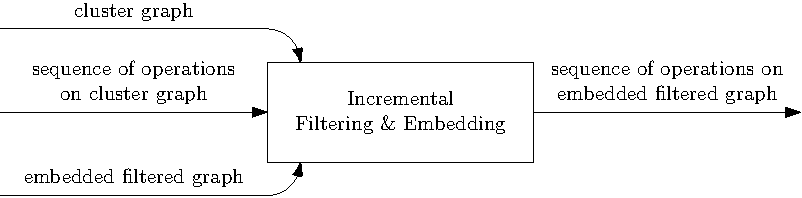
\includegraphics[width=0.9\textwidth]{Resources/DynamicPipeline-IncrementalFilteringAndEmbedding.pdf}
	\caption{Input and output of the incremental filtering and embedding phase.}
	\label{fig:dynamic-pipeline-incremental-filtering-and-embedding}
\end{figure}

Again, we assume that in concrete implementations, an embedded filtered graph preserves enough information about the graphs it was created from to allow for changes of the underlying cluster graph to be incorporated in this phase.

We support the following class of primitive operations on embedded filtered graphs. For all primitive operations that create new vertices or edges the weights can be chosen arbitrarily:
%
\begin{itemize}
	\item \textbf{Insert vertex in an internal face:} We can place a new vertex inside one of the internal faces (which are triangles). In order to preserve the internal triangulatedness of the graph, edges to the three vertices on said face must be added in conjunction and the edges must be embedded such that they do not cross. This operation essentially replaces an internal face with three new triangles.
\begin{figure}[H]
	\centering
	\subfigure[]{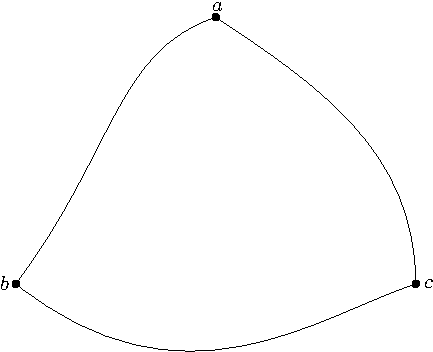
\includegraphics[height=30mm]{Resources/IncrementalFilteringAndEmbedding-InsertVertexInside-Initial.pdf}}
	\quad
	\subfigure[]{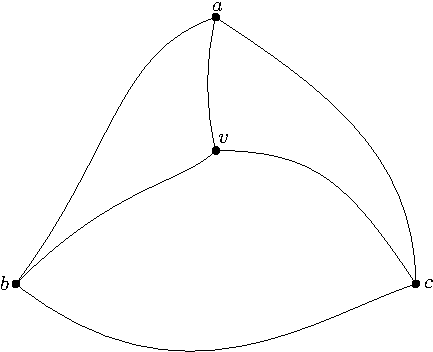
\includegraphics[height=30mm]{Resources/IncrementalFilteringAndEmbedding-InsertVertexInside-Valid.pdf}}
	\quad
	\subfigure[]{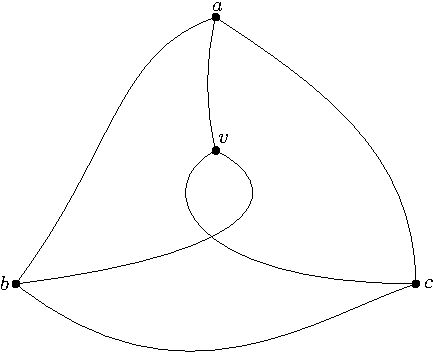
\includegraphics[height=30mm]{Resources/IncrementalFilteringAndEmbedding-InsertVertexInside-Invalid.pdf}}
	\caption{Inserting a vertex in an internal face of a embedded filtered graph (a) correctly (b) and incorrectly, introducing a crossing of the edges $\{b,v\}$, $\{c,v\}$ (c).}
	\label{fig:transformation}
\end{figure}

	\clearpage
	\item \textbf{Insert vertex in outer face:} We can also place a new vertex inside the outer face. The new vertex must be connected to at least two vertices on the outer face (to preserve 2-connectivity), and its adjacent vertices must form a simple path along the original outer face (to preserve internal triangulatedness).
\begin{figure}[H]
	\centering
	\subfigure[]{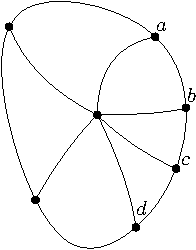
\includegraphics[height=30mm]{Resources/IncrementalFilteringAndEmbedding-InsertVertexOutside-Initial.pdf}}
	\quad
	\subfigure[]{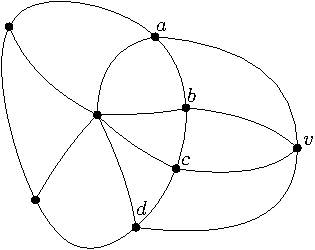
\includegraphics[height=30mm]{Resources/IncrementalFilteringAndEmbedding-InsertVertexOutside-Valid.pdf}}
	\quad
	\subfigure[]{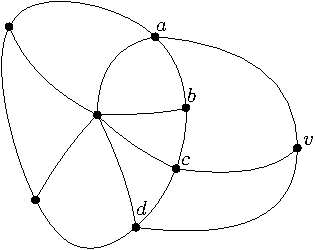
\includegraphics[height=30mm]{Resources/IncrementalFilteringAndEmbedding-InsertVertexOutside-Invalid.pdf}}
	\caption{Inserting a vertex in the outer face of an embedded filtered graph (a) correctly (b) and incorrectly, creating a 4-hole $abcv$ (c).}
	\label{fig:transformation}
\end{figure}

	\item \textbf{Remove internal vertex:} We can only remove internal vertices along with their incident edges if they have degree 3. Such vertices are incident to three pairwise incident triangular faces and their removal would fuse the three triangles together to form a new triangular face.
\begin{figure}[H]
	\centering
	\subfigure[]{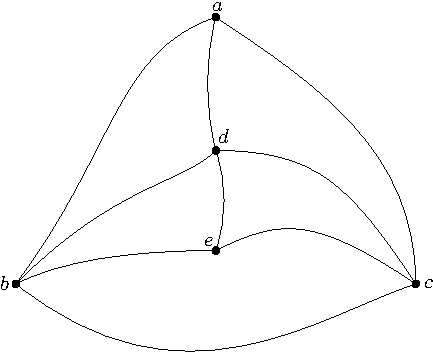
\includegraphics[height=30mm]{Resources/IncrementalFilteringAndEmbedding-RemoveInternalVertex-Initial.pdf}}
	\quad
	\subfigure[]{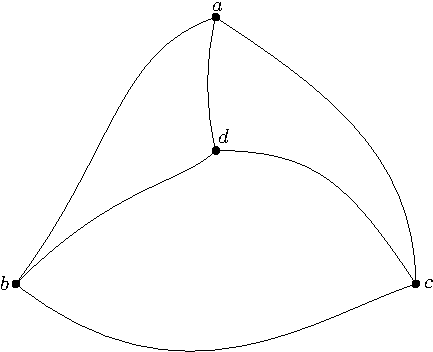
\includegraphics[height=30mm]{Resources/IncrementalFilteringAndEmbedding-RemoveInternalVertex-Valid.pdf}}
	\quad
	\subfigure[]{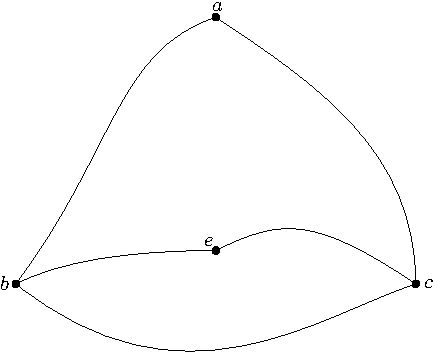
\includegraphics[height=30mm]{Resources/IncrementalFilteringAndEmbedding-RemoveInternalVertex-Invalid.pdf}}
	\caption{Removing an internal vertex of an embedded filtered graph (a) correctly (b) and incorrectly, creating a 4-hole $abec$ (c).}
	\label{fig:transformation}
\end{figure}

	\item \textbf{Remove vertex on outer face:} Vertices on the outer face can be removed along with their incident edges as long as the resulting graph remains 2-connected.
\begin{figure}[H]
	\centering
	\subfigure[]{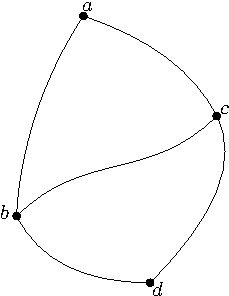
\includegraphics[height=30mm]{Resources/IncrementalFilteringAndEmbedding-RemoveOuterVertex-Initial.pdf}}
	\quad
	\subfigure[]{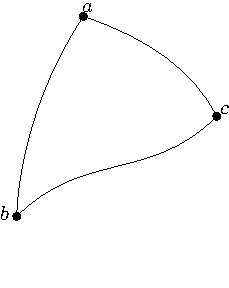
\includegraphics[height=30mm]{Resources/IncrementalFilteringAndEmbedding-RemoveOuterVertex-Valid.pdf}}
	\quad
	\subfigure[]{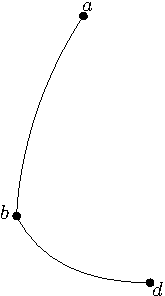
\includegraphics[height=30mm]{Resources/IncrementalFilteringAndEmbedding-RemoveOuterVertex-Invalid.pdf}}
	\caption{Removing a vertex on the outer face of an embedded filtered graph (a) correctly (b) and incorrectly, creating a cut vertex $b$ (c).}
	\label{fig:transformation}
\end{figure}

	\clearpage
	\item \textbf{Flip internal edge:} Internal edges $\{u, v\}$ can be flipped unless their two incident triangles \quoted{tips} $w, x$ are already adjacent. This operation replaces the edge $\{u, v\}$ with the edge $\{w, x\}$ and would therefore create an unwanted duplicate adjacency if $w$ and $x$ were already adjacent.
\begin{figure}[H]
	\centering
	\subfigure[]{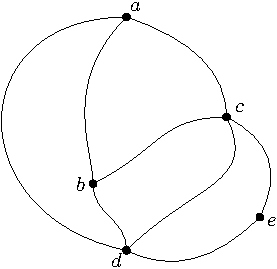
\includegraphics[height=30mm]{Resources/IncrementalFilteringAndEmbedding-FlipInternalEdge-Initial.pdf}}
	\quad
	\subfigure[]{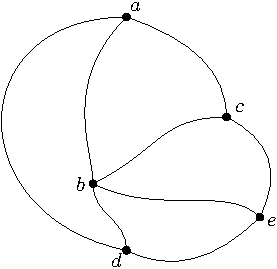
\includegraphics[height=30mm]{Resources/IncrementalFilteringAndEmbedding-FlipInternalEdge-Valid.pdf}}
	\quad
	\subfigure[]{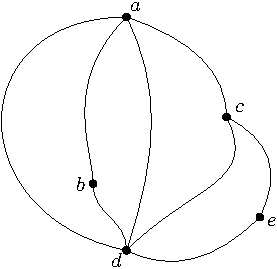
\includegraphics[height=30mm]{Resources/IncrementalFilteringAndEmbedding-FlipInternalEdge-Invalid.pdf}}
	\caption{Flipping an internal edge of an embedded filtered graph (a) correctly (b) and incorrectly, creating a duplicate adjacency between $a$ and $d$ (c).}
	\label{fig:transformation}
\end{figure}

	\item \textbf{Insert edge on outer face:} Edges between nonadjacent vertices $u, v$ on the outer face may only be inserted if they preserve the graph's internal triangulatedness, \ie{} they don't create holes in the graph. Adding such an edge creates a new internal face and is therefore only possible iff $u$ and $v$ have a neighbor in common.
\begin{figure}[H]
	\centering
	\subfigure[]{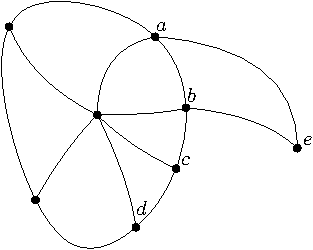
\includegraphics[height=30mm]{Resources/IncrementalFilteringAndEmbedding-InsertOuterEdge-Initial.pdf}}
	\quad
	\subfigure[]{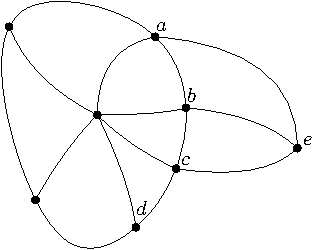
\includegraphics[height=30mm]{Resources/IncrementalFilteringAndEmbedding-InsertOuterEdge-Valid.pdf}}
	\quad
	\subfigure[]{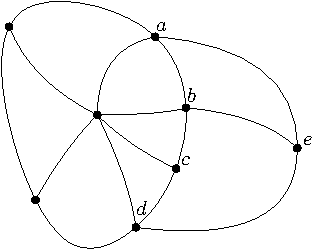
\includegraphics[height=30mm]{Resources/IncrementalFilteringAndEmbedding-InsertOuterEdge-Invalid.pdf}}
	\caption{Inserting an edge on the outer face of an embedded filtered graph (a) correctly (b) and incorrectly, creating a 4-hole $bcde$ (c).}
	\label{fig:transformation}
\end{figure}

	\item \textbf{Remove edge on outer face:} Similarly, we can remove an edge $\{u, v\}$ on the outer face only if it doesn't create holes in the graph. This is the case iff $u$ and $v$ share a neighbor. The graph must also remain 2-connected.
\begin{figure}[H]
	\centering
	\subfigure[]{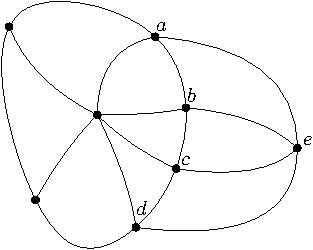
\includegraphics[height=30mm]{Resources/IncrementalFilteringAndEmbedding-RemoveOuterEdge-Initial.pdf}}
	\quad
	\subfigure[]{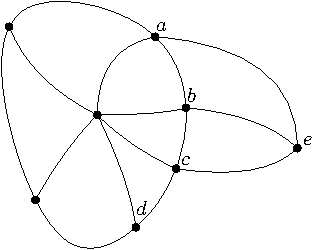
\includegraphics[height=30mm]{Resources/IncrementalFilteringAndEmbedding-RemoveOuterEdge-Valid.pdf}}
	\quad
	\subfigure[]{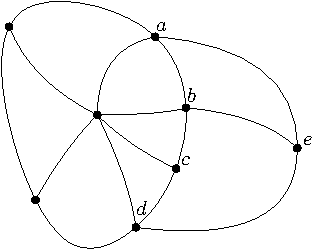
\includegraphics[height=30mm]{Resources/IncrementalFilteringAndEmbedding-RemoveOuterEdge-Invalid.pdf}}
	\caption{Removing an edge on the outer face of an embedded filtered graph (a) correctly (b) and incorrectly, creating a 4-hole $bcde$ (c).}
	\label{fig:transformation}
\end{figure}

	\item \textbf{Update vertex or edge weight:} Of course, we can also set existing vertices' or edges' weights to arbitrary new values.
\end{itemize}
